\section{Experimental Design}
\label{s:experiments-design}

\begin{table*}
\centering
\scalebox{0.9}{
\begin{tabular}{lll} 
\hline
\toprule
\textbf{Feature}                                    & \textbf{Brower features}                     & \textbf{Description of the features}                                                                                                                                                                             \\ 
\hline
\multirow{8}{*}{History features}            & kUrlHistoryVisitCount               & Number of visits to that URL stored in the browser history                                                                                                                                              \\
                                             & kUrlHistoryTypedCount               & Number of times the URL was typed in the Omnibox                                                                                                                                                        \\
                                             & kUrlHistoryLinkCount                & Number of times the URL was reached by clicking a link                                                                                                                                                  \\
                                             & kUrlHistoryVisitCountMoreThan24hAgo & Number of times URL was visited more than 24h ago                                                                                                                                                       \\
                                             & kHttpHostVisitCount                 & \multirow{2}{*}{\begin{tabular}[c]{@{}l@{}}Number of user-visible visits to all URLs on the same host/port as\\~the URL for HTTP and HTTPS \end{tabular}}                                               \\
                                             & kHttpsHostVisitCount                &                                                                                                                                                                                                         \\
                                             & kFirstHttpHostVisitMoreThan24hAgo   & \multirow{2}{*}{\begin{tabular}[c]{@{}l@{}}Boolean feature which is true if the host was visited for the first~\\time more than 24h ago (only considers user-visible visits like above) \end{tabular}}  \\
                                             & kFirstHttpsHostVisitMoreThan24hAgo  &                                                                                                                                                                                                         \\ 
\hline
\multirow{13}{*}{Browse features           } & kHostPrefix                         & \begin{tabular}[c]{@{}l@{}}prefixes appended to~features that tell for which page type\\~the feature pertains\end{tabular}                                                                              \\
                                             & kReferrer                           & Referrer                                                                                                                                                                                                \\
                                             & kHasSSLReferrer                     & True if the referrer was stripped because it is an SSL referrer                                                                                                                                         \\
                                             & kPageTransitionType                 & Stores the page transition                                                                                                                                                                              \\
                                             & kIsFirstNavigation                  & True if this navigation is the first for this tab                                                                                                                                                       \\
                                             & kRedirectUrlMismatch                & \begin{tabular}[c]{@{}l@{}}Feature that is set if the URL from the navigation entry doesn't match\\~the~URL at the end of the redirect chain\end{tabular}                                               \\
                                             & kRedirect                           & The redirect chain that leads to the named page                                                                                                                                                         \\
                                             & kSecureRedirectValue                & \begin{tabular}[c]{@{}l@{}}If a redirect is SSL, we will use this value instead of the actual redirect\\~so we don't leak any SSL sites\end{tabular}                                                    \\
                                             & kHttpStatusCode                     & The HTTP status code for the main document                                                                                                                                                              \\ 
\cline{2-3}
                                             & kSafeBrowsingMaliciousUrl           & \multirow{4}{*}{Fields from the UnsafeResource if there is~any}                                                                                                                                         \\
                                             & kSafeBrowsingOriginalUrl            &                                                                                                                                                                                                         \\
                                             & kSafeBrowsingIsSubresource          &                                                                                                                                                                                                         \\
                                             & kSafeBrowsingThreatType             &                                                                                                                                                                                                         \\
\hline
\end{tabular}}
\caption{Browser features}
\label{tab:Browser features}
\end{table*}

\subsection{Cracking Client-Side model}

% Since the public knowledge about the structure of google safe browsing client-side anti-phishing is rare, we decided to study this ecosystem by directly investigating Chromium, a development version of the chrome browser.
% To study the structure of google safe browsing client-side anti-phishing, we investigated the Chromium. Chromium is a development version of the Chrome browser

We interpreted the network traffic data as well as reverse-engineered the classifier using dynamic and static analysis on chromium source code to analyze the client-side content-based anti-phishing.
To study the client-side anti-phishing mechanism, we extract the features that this classifier uses for detecting phishing websites. There are two types of features in the client-side anti-phishing mechanism. The first group of features is used by the client-side classifier to compute the website's phishy-ness score. To study the structure of google safe browsing client-side anti-phishing which was neglected in previous studies, we investigated Chromium. Chromium is a development version of the Chrome browser. 

We analyzed the classifier in real-time after opening 100 live phishing websites from Phishtank to extract which features are responsible for detecting the malicious websites. Moreover, the values and weights of those features were estimated.

\begin{table}
\centering
\scalebox{0.83}{
\begin{tabular}{lcc} 
\hline
\toprule
              & {Old Model}                                                                         & {New model}                                                                                         \\ 
\hline
\small{Model version} & \small{5}                                                                                  & \small{5X}                                                                                                \\
\small{Rule Numbers}  & \small{2130}                                                                               & \small{3100}                                                                                              \\
\small{Threshold}     & \begin{tabular}[c]{@{}c@{}}\small{Static}\\\small{Threshold}\textbf{\textit\small{{ = 0.5}}}\\~\end{tabular} & \begin{tabular}[c]{@{}c@{}}\small{Dynamic}\\\small{Current Threshold= 0.8999976} \\~\end{tabular}             \\
\small{Features}      & \small{URL-DOM-Term}                                                                       & \small{URL-DOM-Term-Visual~}                                                                              \\
\small{Phishy-ness~}  & \small{score} \textgreater{}= \small{Threshold}                                                                  & \begin{tabular}[c]{@{}c@{}}\small{score} \textgreater{}= \small{ Threshold} \small{or~}\\\small{Visual Target Match}\end{tabular}  \\
\bottomrule
\end{tabular}}
\caption{Difference between the new model and the old model}
\label{ModelDifference}
\end{table}


\subsubsection{Features} 

Client-side content-based anti-phishing uses two type of features:
\begin{enumerate}
\item Model and page (classifier-related) features Chrome client-side content-based anti-phishing classifier uses three type of features in computing the final score.
    \begin{enumerate}
    \item URL features: This type of features make reference to some attributes of the URL.
    \item DOM Features: Client-side classifier uses the Document Object Model (DOM) elements of the page as some features for computing the phishy-ness score. In table \ref{tab:Dom features}, we show all 13 kinds of DOM features employed by chrome.
    \item Term Features: Client-side classifier uses the terms in the page as a kind of feature. This feature refers to a single word or a combination of multiple words (maximum five words).
\end{enumerate}
\item Browser features: After running the classifier on the web page features by the renderer, if the final score is higher than the threshold browser extracts the browser features. Browser features refer to 21 features that are shown in table \ref{tab:browser features}. Browser appends these features to the classifier results and send the phishing request to the server. These features include history, navigation, redirection and safe browsing related features.
    
\end{enumerate}

% \usepackage{multirow}




\begin{table*}
\centering
\scalebox{0.95}{
\begin{tabular}{lll} 
\toprule
 \small{\textbf{DOM feature type}}                                                           & \small{\textbf{Model DOM features}}  & \small{\textbf{Page DOM features}}                                                                                                                              \\ 
\hline
\multirow{7}{*}{\begin{tabular}[c]{@{}l@{}} \small{DOM HTML}\\\small{form features} \end{tabular}}   & \small{PageHasForms}                 & \small{Page has any form} element                                                                                                                               \\
                                                                                     & \small{PageActionOtherDomainFreq}    & \begin{tabular}[c]{@{}l@{}}\small{The fraction of form elements whose “action" attribute}\\ \small{point URL on a different domain} \end{tabular}      \\
                                                                                     & \small{PageActionURL}                & \begin{tabular}[c]{@{}l@{}}\small{The token feature containing each URL}\\\small{that an “action" attribute points to} \end{tabular}  \\
                                                                                     & \smal{PageHasTextInputs}            & \small{The page has any input type=“text" element}                                                                                                              \\
                                                                                     & \small{PageHasPswdInputs}            & \small{The page has any input type=“password" element}                                                                                                          \\
                                                                                     & \small{PageHasRadioInputs}           & \small{The page has any input type=“radio" element}                                                                                                             \\
                                                                                     & \small{PageHasCheckInputs}           & \small{The page has any input type=“checkbox" element}                                                                                                          \\ 
\hline
\multirow{3}{*}{\begin{tabular}[c]{@{}l@{}} \small{DOM HTML}\\\small{link features} \end{tabular}}   & \small{PageExternalLinksFreq}        & \small{The fraction of links on the page that point}\textasciitilde{} \small{to other domains}                                                                          \\
                                                                                     & \small{PageLinkDomain}               & \small{The token feature containing each external domain that is linked to}                                                                                     \\
                                                                                     & \small{PageSecureLinksFreq}          & \small{The fraction of links on the page that use HTTPS}                                                                                                        \\ 
\hline
\multirow{2}{*}{\begin{tabular}[c]{@{}l@{}} \small{DOM HTML}\\\small{script features} \end{tabular}} & \small{PageNumScriptTagsGTOne}       & \small{The number of script elements on the page is greater than 1?}                                                                                            \\
                                                                                     & \small{PageNumScriptTagsGTSix}       & \small{The number of script elements on the page is greater than 6?}                                                                                            \\ 
\hline
\begin{tabular}[c]{@{}l@{}}\small{Other DOM}\\\small{HTML features} \end{tabular}                    & \small{PageImgOtherDomainFreq}       & \begin{tabular}[c]{@{}l@{}}\small{The fraction of images whose source attribute}\\\small{points to an external domain}\end{tabular}                   \\
\bottomrule
\end{tabular}}
\caption{DOM features}
\label{tab:Dom features}
\end{table*}
%%%%%%%%%%%%%






\subsubsection{Algorithm}

Combining static and dynamic analysis, we extract the classification algorithm. The client-side content-based anti-phishing has two phases:

\begin{enumerate}
    \item Pre-classification: Client-side anti-phishing classification starts with some checks in the pre-classification phase. As shown in figure \ref{fig:Pre-classification}, it classifies only [X]HTML documents and HTTP/S pages. It does not classify any tab in incognito or any  URL in whitelisted by enterprise policies, or any URL is in the local Client-side detection whitelist database, and it does not classify for the private IPs.
    
    \item Main classification: In the first step, the client-side content-based anti-phishing runs a pre-classification on the webpage; after passing these conditions, the main classification starts. Client-side suppose Safe Browsing client-side phishing detector distinguishes that the webpage is similar to phishing pages according to the client-side detector machine learning model's results. In that case, it will send a request to the Safe Browsing server to ask the server to make a final decision about the page. If Safe browsing detects the page as a phishing page, the browser shows a warning page.

\begin{figure}[!h]
\centering
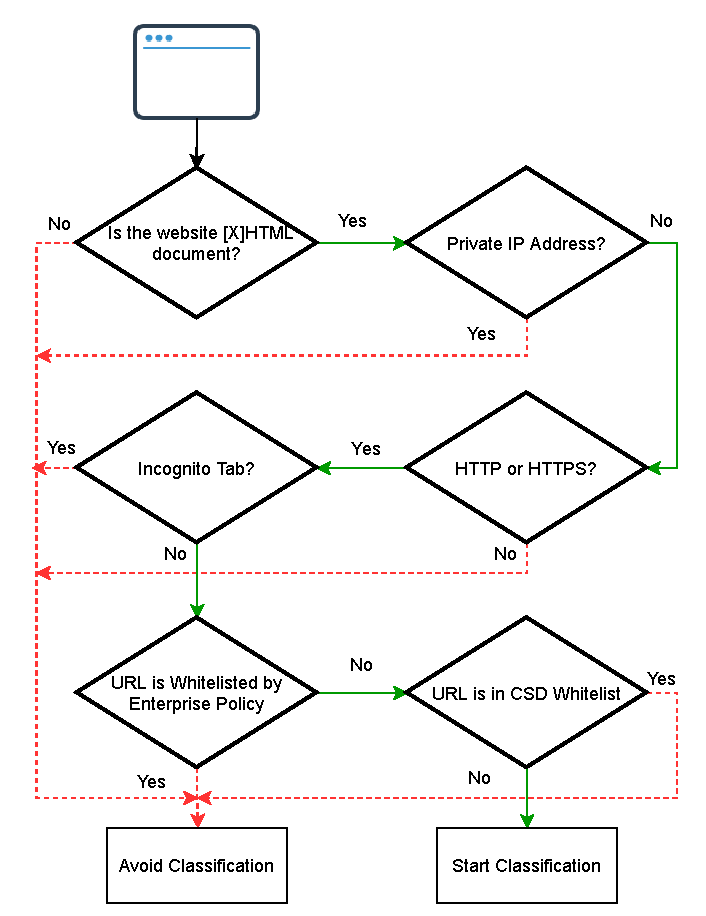
\includegraphics[height=4.5in, width=3in]{figures/preclassificationdiagram-3.pdf}
\caption{Pre-Classification algorithm}
\label{fig:Pre-classification}
\end{figure} 
We found out that the classifier's algorithm has changed compared to the findings of the previous work during our analysis.
Client-side classifier extracts the third type of features, which is called visual features.  It downloads the client-side model's visual target map and compares the visual features with the visual targets. If the features match, the client-side content-based anti-phishing supposes the site as a malicious website and sends the request to the server-side to analyze the site.
\end{enumerate}

\begin{figure}[h!]
\centering
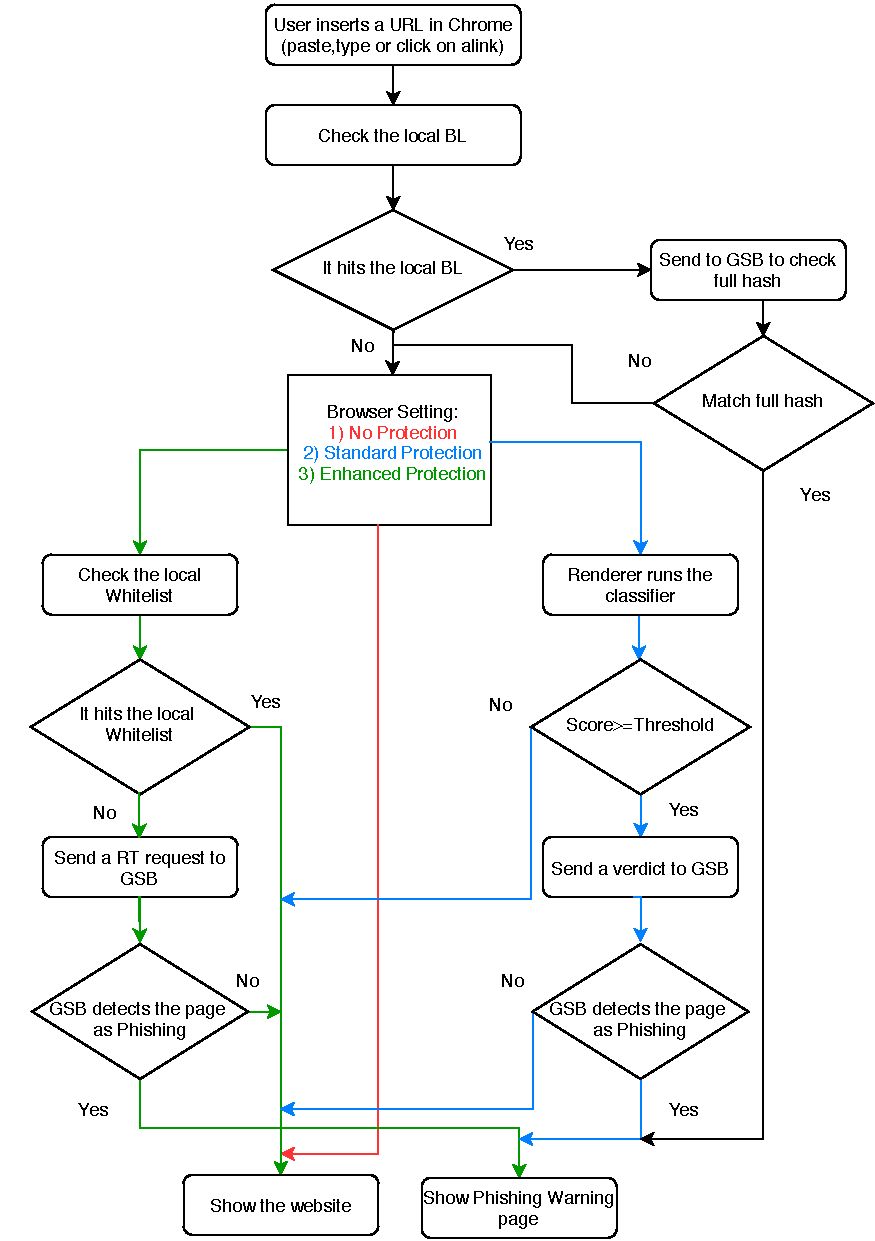
\includegraphics[height=5.0in, width=2.9in]{figures/chrome-ecosystem.pdf}
\caption{Chrome Client-side anti-phishing ecosystem}
\label{fig:Chrome client side anti-phishing flowchart}
\end{figure} 

In the new version of client-side content-based anti-phishing, the classifier uses visual features. As shown in figure \ref{fig:visual features} The classifier detects the related website as a malicious website in two conditions: (1) If the score of the website is above the threshold or (2) If the visual features match the visual target
% \begin{enumerate}
%     \item If the score of the website is above the threshold
%     \item If the visual features match the visual target
% \end{enumerate}

 \begin{figure}[h!]
\centering
\scalebox{0.9}{
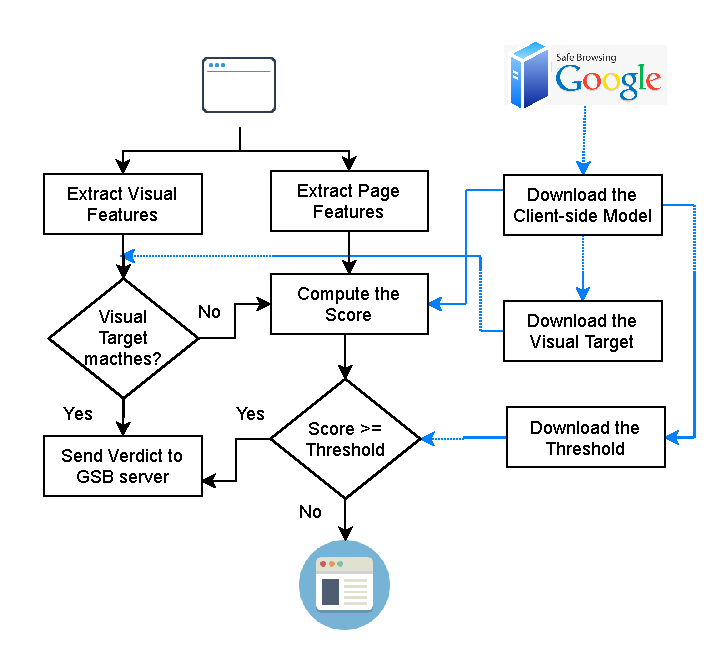
\includegraphics[height=3.7in, width=3.5in]{figures/Visual target (1).pdf}}
\caption{Visual features' role in client-side content-based anti-phishing}
\label{fig:visual features}
\end{figure} 

\subsection{Evaluating client-side Classifier Results}
To measure the client-side content-based anti-phishing, we extracted the classifier, analyzed it with a bunch of phishing websites, and recorded the classifier's final decision besides the scorer's results.
We used 100 phishing websites from Phishtank database for this purpose.
We ensured that similar phishing websites were not duplicated across these URLs.

\subsection{Evaluating Server-Side Classifier Results}
%we show the performance of client-side content based anti-phishing system
To evaluate the server-side classifier, we send many live phishing websites to the server-side classifier and analyzed the server's response to the client. For this purpose, we Modified the phishing threshold to zero to make the browser send the request to the server-side. At technical level,  we modified the threshold in the source code and recompiled the Chromium binary file, visited 100 phishing websites, and captured the server responses using a proxy. For making more promising decision, we recorded the client-side classifier scores of all the phishing websites.

\subsection{Password Protection Anti-phishing}
We analyze the phishing websites' HTML files that we fed to the client-side password-protection anti-phishing during our experiment. After performing hybrid analysis on chromium source code and monitoring the network data with BurpSuit proxy beside this analysis, we found out this mechanism has a significant weakness. If the DOM element name in the page is not ``password", the password protection does not carry out a password-exposure check nor phishing classification for that page.  
\subsection{Real-time Anti-phishing evaluation}

In September 2019, chrome version 79 came with a new defense layer against phishing websites. Google to cover the blacklist refreshing windows and preventing the attackers from exploiting that approximately 30 minutes refreshing time to perform their new attacks, or continue their attacks by continuously changing their domains, presented the real-time anti-phishing method.
Having chrome version 79 or newer, when users visit a website, Chrome checks it against the whitelist database on the user's system. 
In Chrome version 79 or newer, Chrome sends the URL to safe browsing unless it is on a whitelist. The whitelist is stored locally and includes thousands of popular websites that are known to be safe. If the visited website's URL does not match with the local whitelist database, the browser sends the URL to the google safe browsing server to check if the user is visiting a malicious website.~\cite{gsbapi,googlechromeprivacywhitepaper}. 
In this study, we consider real-time in the browser settings in the blacklisting experiment to evaluate its effect on blacklisting performance.
% coverage and speed. 
We also evaluate the empirical experiment on 50 phishing websites and monitor the chrome behavior, the real-time request that the browser sends, and the server results.

\subsection{Measuring Blacklist performance}
%{Speed and Coverage}
%we show the content-based anti-phishing effects on blacklisting coverage and speed
It is the central part of the experiment:
For the 14 batches domains, we use different combinations of the browser-side anti-phishing mechanisms, cloaking, and reporting to evaluate the effects of client-side anti-phishing methods, including client-side content-based and real-time anti-phishing, cloaking as the most popular evasion method and reporting on the blacklisting performance.
% speed and coverage.

This analysis seeks to figure out how effective client-side content-based anti-phishing is in blacklisting and protecting the user from phishing websites. Also, How effective client-side content-based anti-phishing is in dealing with cloaking as an evasion technique.

\subsection{Privacy Issues in Client-Side Anti-Phishing }

In the phishing context, attackers need to gain user's sensitive and private information. However, anti-phishing techniques like Google Safe Browsing client-side anti-phishing claims that it protects user's sensitive information~\cite{googlechromeprivacywhitepaper}, but in reality, Chrome browser does not give the true sense of trust to the users and does not entirely guarantee the privacy of the user's activities.
We analyze client-side anti-phishing behavior in user privacy in two different scenarios:
\begin{enumerate}
    \item User privacy in phishing detection for every un-seen website
    \item User privacy in password protection mechanism
\end{enumerate}

\subsubsection{Privacy issue in client-side anti-phishing detection} 

When the client-side anti-phishing classifier computes the page's phishy-ness score, the pages with a score above the threshold browser send a request to the server to check the page and respond with the final decision about the page's phishy-ness score. 
Our experiments show that this request includes the page URL, referring URL, as well as technical parameters about the classifier and classification results such as:
1) Feature Map
2) Client Score
3) Model version
4) Browser features
5) URL
6) The client-side classifier result
7) Vision match result
8) Feature map size
9) Non-model feature map
10) Non-model feature map size
11) Referrer URL
12) Shingle hashes size
13) Shingle hashes
14) Model file name
This request includes the visited URL.
% Figure~\ref{fig:Phishing Request to the server} shows a screenshot of proxy showing the sent phishing request to the Google Safe Browsing. 
However, google chrome informs the user about the information it sends to the server under the related setting.

\subsubsection{Privacy issue in client-side password protection }
Password protection is not enabled on the chrome browser setting. Having chosen this protection by the user, if a user clicks on the password box, client-side password protection starts running phishing classification on the page regardless of previous pre-classification results~\cite{mardini_2019}. 
Our experiments show that when users insert a password, the browser sends the visited URL and URLs of all the websites with the same saved password to google safe browsing.   
However, the client-side password protection mechanism eliminates user's information includes user names and passwords. It exposes users' current and previous activities related to the password to the google safe browsing server. The revealed privacy issue is not disclosed to the user in the chrome browser settings where the user should enable this mechanism.

\section{Implementation of Experiments}
In the preliminary experiment, we extracted a total of 200 newest and not blacklisted phishing websites 10 per week from the Phishtank database, 100 for the client-side analysis, and 100 for server-side classifier evaluation. 
For the blacklisting experiment, we adjusted a previously-conducted test framework(Phishfarm \cite{oest2019phishfarm}) to establish our needed phishing websites.
To empirically measure blacklisting coverage and speed
and evaluate browser-based defenses such as blacklisting, content-based, and real-time anti-phishing, the testbed facilitates the configuration, development, API-based reporting, and monitoring of the nondangerous phishing websites.  We enhanced the testbed to support automation of monitoring the network, cloaking, and API-based reporting to accurately imitate current phishing trends and ecosystem defenses.

\subsection{Overview}

Our experiment is divided into the following steps: 
First, we designed 14 groups to entirely cover the features we want to evaluate their effects on the blacklisting process. Second deployed phishing websites using Phishfarm test-bed, 
To reduce the chances of being blacklisted due to the domain's low reputation, we used the domains a month later.
We deploy the network monitor tools in the VMs, then activated the websites. Over the next seven days, we monitor the blacklist status, and we log the crawler traffic.
At the last step of the blacklist experiment, we deactivated the websites and analyzed the log file.

\subsection{Client-side and server-side Classifier evaluation}

As an open-source project, we are able to compile chromium source code to achieve a debug version, including symbols of functions, variables, algorithms, databases, and structures. In this paper, we use visual studio as the debug tool. We explore the Safe Browsing folder in the source code to locate client-side anti-phishing files, data structures, and debugging points. 
The multi-layer architecture prevents to crack all anti-phishing components by static analysis. Extracting model and page features, setting threshold, computing the score, and checking the visual target matches are accrued in the renderer process. On the other hand, pre-classification checks, loading machine learning model, password protection process, browser feature extraction, Sending the classification request to the renderer process, receiving the results, and finally sending phishing requests to the server are implemented in the browser process.
We omitted some extracted sensitive details of chrome client-side anti-phishing intentionally to prevent them from being used by malicious users. 

\subsection{Blacklist Monitoring}

To empirically monitor blacklisting speed and coverage
of phishing websites, We used the adapted previous-presented test-framework( Phishfarm) \cite{oest2019phishfarm} on a total of 8 virtual machines(VMs). We modified chrome browser anti-phishing settings on each VM to perform a blacklisting monitor with different anti-phishing techniques.

\subsection{Network Monitoring}

To study privacy-related issues in the client-side content-based anti-phishing, we implement a proxy to monitor the network during the blacklist experiment. We used BurpSuit for the windows platform in the preliminary experiment and MITMproxy during the main experiment on the Ubuntu systems. To verify that no traffic bypassed the proxy in the chrome browser, we also employed Wireshark to capture network data.
 
\begin{table*}[t]
\centering
\scalebox{0.95}{
\begin{tabular}{ccccccccc} 
\hline
\toprule
                     & \multicolumn{5}{c}{Experiment Settings}                                                                                                                                                            & \multirow{4}{*}{\begin{tabular}[c]{@{}c@{}}Total Number of\\Websites per group\end{tabular}} & \multirow{4}{*}{\begin{tabular}[c]{@{}c@{}}Number of\\Blacklisted\\websites:\\Desktop chrome\end{tabular}} & \multirow{4}{*}{\begin{tabular}[c]{@{}c@{}}Number of\\Blacklisted\\websites:\\Mobile chrome\end{tabular}}  \\ 
\cline{1-6}
                     & \multirow{3}{*}{URL~} & \multirow{3}{*}{CB} & \multirow{3}{*}{RT} & \multirow{3}{*}{Report~} & \multirow{3}{*}{Evasion Technique}                                                                  &                                                                                              &                                                                                                             &                                                                                                           \\
\multicolumn{1}{l}{} &                       &                     &                     &                          &                                                                                                     &                                                                                              &                                                                                                             &                                                                                                           \\
\multicolumn{1}{l}{} &                       &                     &                     &                          &                                                                                                     &                                                                                              &                                                                                                             &                                                                                                           \\ 
\hline
\small{1}  & \small{Rand} & \cmark & \xmark  & \xmark      & \small{Cloaking}                                                                                            & \small{35}                                                                                           & {\cellcolor[rgb]{1,0.49,0.49}}\small{0}                                                                             & {\cellcolor[rgb]{1,0.49,0.49}}\small{0}                                                                           \\
\small{2}  & \small{Rand} & \cmark &\xmark  & \xmark      & \small{No Cloaking}                                                                                            & \small{35}                                                                                           & {\cellcolor[rgb]{1,0.49,0.49}}\small{0}                                                                             & {\cellcolor[rgb]{1,0.49,0.49}}\small{0}                                                                           \\
\small{3}  & \small{Susp} &  \cmark & \xmark  & \xmark      & \small{No Cloaking}~                                                                                        & \small{35}                                                                                          & {\cellcolor[rgb]{1,0.49,0.49}}\small{0}                                                                             & {\cellcolor[rgb]{1,0.49,0.49}}\small{0}                                                                           \\
\small{4}  & \small{Rand} &  \cmark &  \cmark & \xmark      & \small{No Cloaking}                                                                                        &  \small{35}                                                                                           & {\cellcolor[rgb]{1,0.49,0.49}}\small{0}                                                                             & {\cellcolor[rgb]{1,0.49,0.49}}\small{0}                                                                           \\
\small{5}  & \small{Susp} & \cmark & \cmark & \xmark     & \small{Cloaking}                                                                                             & \small{35}                                                                                           & {\cellcolor[rgb]{1,0.49,0.49}}\small{1}                                                                             & {\cellcolor[rgb]{1,0.49,0.49}}\small{0}                                                                           \\
\small{6}  & \small{Rand} & \cmark & \cmark & \cmark     & \small{No Cloaking}                                                                                         & \small{35}                                                                                           & {\cellcolor[rgb]{0.592,0.867,0.592}}\small{33}                                                                      & {\cellcolor[rgb]{0.592,0.867,0.592}}\small{35}                                                                    \\
\small{7}  & \small{Susp} &\xmark  &  \cmark &  \cmark     & \begin{tabular}[c]{@{}c@{}}\small{Cloaking}\end{tabular} & \small{35}                                                                                           & {\cellcolor[rgb]{0.592,0.867,0.592}}\small{34}                                                                      & {\cellcolor[rgb]{1,0.49,0.49}}\small{0}                                                                           \\
\small{8}  & \small{Susp} & \cmark & \cmark & \cmark     & \small{No Cloaking}                                                                                         & \small{35}                                                                                           & {\cellcolor[rgb]{0.592,0.867,0.592}}\small{34}                                                                      & {\cellcolor[rgb]{0.592,0.867,0.592}}\small{31}                                                                    \\
\small{9}  & \small{Susp} & \cmark & \cmark & \cmark     & \small{No Cloaking}                                                                                         & \small{35}                                                                                           & {\cellcolor[rgb]{0.592,0.867,0.592}}\small{34}                                                                      & {\cellcolor[rgb]{0.592,0.867,0.592}}\small{33}                                                                    \\
\small{10} & \small{Rand} & \cmark & \xmark  & \cmark     & \small{Cloaking}                                                                                             & \small{35}                                                                                           & {\cellcolor[rgb]{0.592,0.867,0.592}}\small{35}                                                                      & {\cellcolor[rgb]{1,0.49,0.49}}\small{0}                                                                           \\
\small{11} & \small{Susp} & \cmark & \xmark  & \cmark     & \small{Cloaking}                                                                                             & \small{35}                                                                                           & {\cellcolor[rgb]{0.592,0.867,0.592}}\small{35}                                                                      & {\cellcolor[rgb]{1,0.49,0.49}}\small{2}                                                                           \\
\small{12} & \small{Rand} & \cmark & \xmark  & \cmark     & \small{No Cloaking}                                                                                         & \small{35}                                                                                           & {\cellcolor[rgb]{0.592,0.867,0.592}}\small{35}                                                                      & {\cellcolor[rgb]{0.592,0.867,0.592}}\small{33}                                                                    \\
\small{13} & \small{Rand} & \xmark  & \cmark & \cmark     & \small{Cloaking}                                                                                             & \small{35}                                                                                           & {\cellcolor[rgb]{0.592,0.867,0.592}}\small{35}                                                                      & {\cellcolor[rgb]{1,0.49,0.49}}\small{0}                                                                           \\
\small{14} & \small{Rand} & \xmark  & \cmark & \cmark     & \begin{tabular}[c]{@{}c@{}}\small{No Cloaking} \\+ \small{Not visible}\\\small{~to the Client-side Classifier}\end{tabular} & \small{35}                                                                                           & {\cellcolor[rgb]{0.592,0.867,0.592}}\small{35}                                                                     & {\cellcolor[rgb]{0.592,0.867,0.592}}\small{31}                                                                   \\
\bottomrule
\end{tabular}}
\caption{Blacklisting coverage results}
\label{fig:coverage results}
\end{table*}